% This file was created with tikzplotlib v0.10.1.
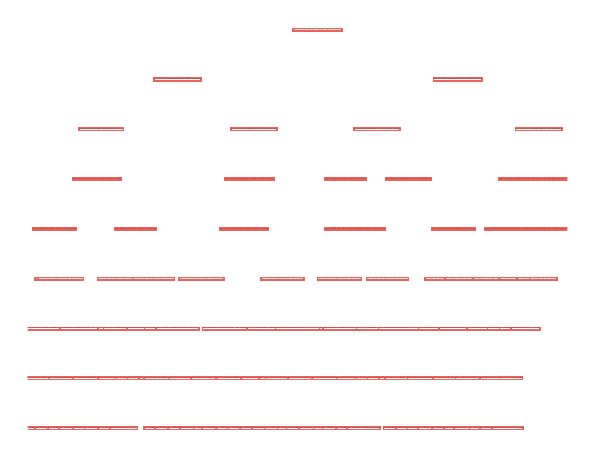
\begin{tikzpicture}

\definecolor{darkgray176}{RGB}{176,176,176}
\definecolor{tomato2369992}{RGB}{236,99,92}

\begin{axis}[
hide x axis,
hide y axis,
tick align=outside,
tick pos=left,
x grid style={darkgray176},
xmin=0, xmax=1,
xtick style={color=black},
y grid style={darkgray176},
ymin=0, ymax=1,
ytick style={color=black}
]
\draw (axis cs:0.0222222222222222,0.0555555555555556) node[
  scale=0.05,
  fill=white,
  draw=tomato2369992,
  line width=0.6pt,
  inner sep=3.6pt,
  text=black,
  rotate=0.0,
  align=center
]{gini = 0.0
samples = 169
value = [169, 0, 0, 0]};
\draw (axis cs:0.0444444444444444,0.0555555555555556) node[
  scale=0.05,
  fill=white,
  draw=tomato2369992,
  line width=0.6pt,
  inner sep=3.6pt,
  text=black,
  rotate=0.0,
  align=center
]{gini = 0.492
samples = 1358
value = [868, 422, 0, 68]};
\draw (axis cs:0.0666666666666667,0.0555555555555556) node[
  scale=0.05,
  fill=white,
  draw=tomato2369992,
  line width=0.6pt,
  inner sep=3.6pt,
  text=black,
  rotate=0.0,
  align=center
]{gini = 0.492
samples = 204
value = [115, 89, 0, 0]};
\draw (axis cs:0.0888888888888889,0.0555555555555556) node[
  scale=0.05,
  fill=white,
  draw=tomato2369992,
  line width=0.6pt,
  inner sep=3.6pt,
  text=black,
  rotate=0.0,
  align=center
]{gini = 0.592
samples = 321
value = [30, 189, 41, 61]};
\draw (axis cs:0.111111111111111,0.0555555555555556) node[
  scale=0.05,
  fill=white,
  draw=tomato2369992,
  line width=0.6pt,
  inner sep=3.6pt,
  text=black,
  rotate=0.0,
  align=center
]{gini = 0.0
samples = 106
value = [106, 0, 0, 0]};
\draw (axis cs:0.133333333333333,0.0555555555555556) node[
  scale=0.05,
  fill=white,
  draw=tomato2369992,
  line width=0.6pt,
  inner sep=3.6pt,
  text=black,
  rotate=0.0,
  align=center
]{gini = 0.479
samples = 63
value = [25, 38, 0, 0]};
\draw (axis cs:0.155555555555556,0.0555555555555556) node[
  scale=0.05,
  fill=white,
  draw=tomato2369992,
  line width=0.6pt,
  inner sep=3.6pt,
  text=black,
  rotate=0.0,
  align=center
]{gini = 0.0
samples = 59
value = [59, 0, 0, 0]};
\draw (axis cs:0.177777777777778,0.0555555555555556) node[
  scale=0.05,
  fill=white,
  draw=tomato2369992,
  line width=0.6pt,
  inner sep=3.6pt,
  text=black,
  rotate=0.0,
  align=center
]{gini = 0.0
samples = 57
value = [0, 57, 0, 0]};
\draw (axis cs:0.244444444444444,0.0555555555555556) node[
  scale=0.05,
  fill=white,
  draw=tomato2369992,
  line width=0.6pt,
  inner sep=3.6pt,
  text=black,
  rotate=0.0,
  align=center
]{gini = 0.0
samples = 2175
value = [2175, 0, 0, 0]};
\draw (axis cs:0.266666666666667,0.0555555555555556) node[
  scale=0.05,
  fill=white,
  draw=tomato2369992,
  line width=0.6pt,
  inner sep=3.6pt,
  text=black,
  rotate=0.0,
  align=center
]{gini = 0.139
samples = 1328
value = [1228, 0, 0, 100]};
\draw (axis cs:0.288888888888889,0.0555555555555556) node[
  scale=0.05,
  fill=white,
  draw=tomato2369992,
  line width=0.6pt,
  inner sep=3.6pt,
  text=black,
  rotate=0.0,
  align=center
]{gini = 0.307
samples = 275
value = [52, 0, 0, 223]};
\draw (axis cs:0.311111111111111,0.0555555555555556) node[
  scale=0.05,
  fill=white,
  draw=tomato2369992,
  line width=0.6pt,
  inner sep=3.6pt,
  text=black,
  rotate=0.0,
  align=center
]{gini = 0.116
samples = 874
value = [820, 0, 0, 54]};
\draw (axis cs:0.333333333333333,0.0555555555555556) node[
  scale=0.05,
  fill=white,
  draw=tomato2369992,
  line width=0.6pt,
  inner sep=3.6pt,
  text=black,
  rotate=0.0,
  align=center
]{gini = 0.0
samples = 29
value = [0, 0, 0, 29]};
\draw (axis cs:0.355555555555556,0.0555555555555556) node[
  scale=0.05,
  fill=white,
  draw=tomato2369992,
  line width=0.6pt,
  inner sep=3.6pt,
  text=black,
  rotate=0.0,
  align=center
]{gini = 0.292
samples = 2698
value = [2251, 265, 93, 89]};
\draw (axis cs:0.377777777777778,0.0555555555555556) node[
  scale=0.05,
  fill=white,
  draw=tomato2369992,
  line width=0.6pt,
  inner sep=3.6pt,
  text=black,
  rotate=0.0,
  align=center
]{gini = 0.652
samples = 183
value = [0, 43, 70, 70]};
\draw (axis cs:0.4,0.0555555555555556) node[
  scale=0.05,
  fill=white,
  draw=tomato2369992,
  line width=0.6pt,
  inner sep=3.6pt,
  text=black,
  rotate=0.0,
  align=center
]{gini = 0.296
samples = 265
value = [220, 0, 23, 22]};
\draw (axis cs:0.422222222222222,0.0555555555555556) node[
  scale=0.05,
  fill=white,
  draw=tomato2369992,
  line width=0.6pt,
  inner sep=3.6pt,
  text=black,
  rotate=0.0,
  align=center
]{gini = 0.201
samples = 493
value = [437, 0, 0, 56]};
\draw (axis cs:0.444444444444444,0.0555555555555556) node[
  scale=0.05,
  fill=white,
  draw=tomato2369992,
  line width=0.6pt,
  inner sep=3.6pt,
  text=black,
  rotate=0.0,
  align=center
]{gini = 0.429
samples = 151
value = [47, 0, 0, 104]};
\draw (axis cs:0.466666666666667,0.0555555555555556) node[
  scale=0.05,
  fill=white,
  draw=tomato2369992,
  line width=0.6pt,
  inner sep=3.6pt,
  text=black,
  rotate=0.0,
  align=center
]{gini = 0.1
samples = 551
value = [522, 0, 0, 29]};
\draw (axis cs:0.488888888888889,0.0555555555555556) node[
  scale=0.05,
  fill=white,
  draw=tomato2369992,
  line width=0.6pt,
  inner sep=3.6pt,
  text=black,
  rotate=0.0,
  align=center
]{gini = 0.0
samples = 45
value = [0, 0, 0, 45]};
\draw (axis cs:0.511111111111111,0.0555555555555556) node[
  scale=0.05,
  fill=white,
  draw=tomato2369992,
  line width=0.6pt,
  inner sep=3.6pt,
  text=black,
  rotate=0.0,
  align=center
]{gini = 0.663
samples = 572
value = [267, 39, 100, 166]};
\draw (axis cs:0.533333333333333,0.0555555555555556) node[
  scale=0.05,
  fill=white,
  draw=tomato2369992,
  line width=0.6pt,
  inner sep=3.6pt,
  text=black,
  rotate=0.0,
  align=center
]{gini = 0.498
samples = 407
value = [84, 13, 37, 273]};
\draw (axis cs:0.555555555555556,0.0555555555555556) node[
  scale=0.05,
  fill=white,
  draw=tomato2369992,
  line width=0.6pt,
  inner sep=3.6pt,
  text=black,
  rotate=0.0,
  align=center
]{gini = 0.0
samples = 51
value = [51, 0, 0, 0]};
\draw (axis cs:0.577777777777778,0.0555555555555556) node[
  scale=0.05,
  fill=white,
  draw=tomato2369992,
  line width=0.6pt,
  inner sep=3.6pt,
  text=black,
  rotate=0.0,
  align=center
]{gini = 0.182
samples = 1791
value = [102, 0, 1615, 74]};
\draw (axis cs:0.6,0.0555555555555556) node[
  scale=0.05,
  fill=white,
  draw=tomato2369992,
  line width=0.6pt,
  inner sep=3.6pt,
  text=black,
  rotate=0.0,
  align=center
]{gini = 0.352
samples = 149
value = [0, 0, 115, 34]};
\draw (axis cs:0.622222222222222,0.0555555555555556) node[
  scale=0.05,
  fill=white,
  draw=tomato2369992,
  line width=0.6pt,
  inner sep=3.6pt,
  text=black,
  rotate=0.0,
  align=center
]{gini = 0.048
samples = 1772
value = [0, 0, 1728, 44]};
\draw (axis cs:0.688888888888889,0.0555555555555556) node[
  scale=0.05,
  fill=white,
  draw=tomato2369992,
  line width=0.6pt,
  inner sep=3.6pt,
  text=black,
  rotate=0.0,
  align=center
]{gini = 0.479
samples = 256
value = [0, 0, 102, 154]};
\draw (axis cs:0.711111111111111,0.0555555555555556) node[
  scale=0.05,
  fill=white,
  draw=tomato2369992,
  line width=0.6pt,
  inner sep=3.6pt,
  text=black,
  rotate=0.0,
  align=center
]{gini = 0.313
samples = 232
value = [45, 0, 187, 0]};
\draw (axis cs:0.733333333333333,0.0555555555555556) node[
  scale=0.05,
  fill=white,
  draw=tomato2369992,
  line width=0.6pt,
  inner sep=3.6pt,
  text=black,
  rotate=0.0,
  align=center
]{gini = 0.571
samples = 182
value = [103, 0, 24, 55]};
\draw (axis cs:0.755555555555556,0.0555555555555556) node[
  scale=0.05,
  fill=white,
  draw=tomato2369992,
  line width=0.6pt,
  inner sep=3.6pt,
  text=black,
  rotate=0.0,
  align=center
]{gini = 0.47
samples = 2533
value = [386, 48, 1772, 327]};
\draw (axis cs:0.777777777777778,0.0555555555555556) node[
  scale=0.05,
  fill=white,
  draw=tomato2369992,
  line width=0.6pt,
  inner sep=3.6pt,
  text=black,
  rotate=0.0,
  align=center
]{gini = 0.32
samples = 275
value = [0, 0, 220, 55]};
\draw (axis cs:0.8,0.0555555555555556) node[
  scale=0.05,
  fill=white,
  draw=tomato2369992,
  line width=0.6pt,
  inner sep=3.6pt,
  text=black,
  rotate=0.0,
  align=center
]{gini = 0.068
samples = 743
value = [0, 0, 717, 26]};
\draw (axis cs:0.822222222222222,0.0555555555555556) node[
  scale=0.05,
  fill=white,
  draw=tomato2369992,
  line width=0.6pt,
  inner sep=3.6pt,
  text=black,
  rotate=0.0,
  align=center
]{gini = 0.613
samples = 1634
value = [313, 866, 431, 24]};
\draw (axis cs:0.844444444444444,0.0555555555555556) node[
  scale=0.05,
  fill=white,
  draw=tomato2369992,
  line width=0.6pt,
  inner sep=3.6pt,
  text=black,
  rotate=0.0,
  align=center
]{gini = 0.0
samples = 35
value = [0, 0, 0, 35]};
\draw (axis cs:0.866666666666667,0.0555555555555556) node[
  scale=0.05,
  fill=white,
  draw=tomato2369992,
  line width=0.6pt,
  inner sep=3.6pt,
  text=black,
  rotate=0.0,
  align=center
]{gini = 0.45
samples = 211
value = [0, 0, 139, 72]};
\draw (axis cs:0.888888888888889,0.0555555555555556) node[
  scale=0.05,
  fill=white,
  draw=tomato2369992,
  line width=0.6pt,
  inner sep=3.6pt,
  text=black,
  rotate=0.0,
  align=center
]{gini = 0.627
samples = 155
value = [38, 77, 40, 0]};
\draw (axis cs:0.0111111111111111,0.166666666666667) node[
  scale=0.05,
  fill=white,
  draw=tomato2369992,
  line width=0.6pt,
  inner sep=3.6pt,
  text=black,
  rotate=0.0,
  align=center
]{gini = 0.0
samples = 72
value = [72, 0, 0, 0]};
\draw (axis cs:0.0333333333333333,0.166666666666667) node[
  scale=0.05,
  fill=white,
  draw=tomato2369992,
  line width=0.6pt,
  inner sep=3.6pt,
  text=black,
  rotate=0.0,
  align=center
]{X[1] <= 153.125
gini = 0.46
samples = 1527
value = [1037, 422, 0, 68]};
\draw (axis cs:0.0777777777777778,0.166666666666667) node[
  scale=0.05,
  fill=white,
  draw=tomato2369992,
  line width=0.6pt,
  inner sep=3.6pt,
  text=black,
  rotate=0.0,
  align=center
]{X[0] <= 281.23
gini = 0.624
samples = 525
value = [145, 278, 41, 61]};
\draw (axis cs:0.122222222222222,0.166666666666667) node[
  scale=0.05,
  fill=white,
  draw=tomato2369992,
  line width=0.6pt,
  inner sep=3.6pt,
  text=black,
  rotate=0.0,
  align=center
]{X[1] <= 477.545
gini = 0.349
samples = 169
value = [131, 38, 0, 0]};
\draw (axis cs:0.166666666666667,0.166666666666667) node[
  scale=0.05,
  fill=white,
  draw=tomato2369992,
  line width=0.6pt,
  inner sep=3.6pt,
  text=black,
  rotate=0.0,
  align=center
]{X[0] <= 285.045
gini = 0.5
samples = 116
value = [59, 57, 0, 0]};
\draw (axis cs:0.188888888888889,0.166666666666667) node[
  scale=0.05,
  fill=white,
  draw=tomato2369992,
  line width=0.6pt,
  inner sep=3.6pt,
  text=black,
  rotate=0.0,
  align=center
]{gini = 0.0
samples = 61
value = [0, 61, 0, 0]};
\draw (axis cs:0.211111111111111,0.166666666666667) node[
  scale=0.05,
  fill=white,
  draw=tomato2369992,
  line width=0.6pt,
  inner sep=3.6pt,
  text=black,
  rotate=0.0,
  align=center
]{gini = 0.0
samples = 23
value = [0, 23, 0, 0]};
\draw (axis cs:0.233333333333333,0.166666666666667) node[
  scale=0.05,
  fill=white,
  draw=tomato2369992,
  line width=0.6pt,
  inner sep=3.6pt,
  text=black,
  rotate=0.0,
  align=center
]{gini = 0.0
samples = 116
value = [0, 0, 0, 116]};
\draw (axis cs:0.255555555555556,0.166666666666667) node[
  scale=0.05,
  fill=white,
  draw=tomato2369992,
  line width=0.6pt,
  inner sep=3.6pt,
  text=black,
  rotate=0.0,
  align=center
]{X[2] <= 253.62
gini = 0.055
samples = 3503
value = [3403, 0, 0, 100]};
\draw (axis cs:0.3,0.166666666666667) node[
  scale=0.05,
  fill=white,
  draw=tomato2369992,
  line width=0.6pt,
  inner sep=3.6pt,
  text=black,
  rotate=0.0,
  align=center
]{X[2] <= 556.93
gini = 0.366
samples = 1149
value = [872, 0, 0, 277]};
\draw (axis cs:0.344444444444444,0.166666666666667) node[
  scale=0.05,
  fill=white,
  draw=tomato2369992,
  line width=0.6pt,
  inner sep=3.6pt,
  text=black,
  rotate=0.0,
  align=center
]{X[1] <= 29.755
gini = 0.306
samples = 2727
value = [2251, 265, 93, 118]};
\draw (axis cs:0.388888888888889,0.166666666666667) node[
  scale=0.05,
  fill=white,
  draw=tomato2369992,
  line width=0.6pt,
  inner sep=3.6pt,
  text=black,
  rotate=0.0,
  align=center
]{X[3] <= 177.715
gini = 0.664
samples = 448
value = [220, 43, 93, 92]};
\draw (axis cs:0.433333333333333,0.166666666666667) node[
  scale=0.05,
  fill=white,
  draw=tomato2369992,
  line width=0.6pt,
  inner sep=3.6pt,
  text=black,
  rotate=0.0,
  align=center
]{X[3] <= 52.55
gini = 0.373
samples = 644
value = [484, 0, 0, 160]};
\draw (axis cs:0.455555555555556,0.166666666666667) node[
  scale=0.05,
  fill=white,
  draw=tomato2369992,
  line width=0.6pt,
  inner sep=3.6pt,
  text=black,
  rotate=0.0,
  align=center
]{gini = 0.0
samples = 545
value = [545, 0, 0, 0]};
\draw (axis cs:0.477777777777778,0.166666666666667) node[
  scale=0.05,
  fill=white,
  draw=tomato2369992,
  line width=0.6pt,
  inner sep=3.6pt,
  text=black,
  rotate=0.0,
  align=center
]{X[5] <= 210.0
gini = 0.217
samples = 596
value = [522, 0, 0, 74]};
\draw (axis cs:0.522222222222222,0.166666666666667) node[
  scale=0.05,
  fill=white,
  draw=tomato2369992,
  line width=0.6pt,
  inner sep=3.6pt,
  text=black,
  rotate=0.0,
  align=center
]{X[1] <= 38.805
gini = 0.648
samples = 979
value = [351, 52, 137, 439]};
\draw (axis cs:0.566666666666667,0.166666666666667) node[
  scale=0.05,
  fill=white,
  draw=tomato2369992,
  line width=0.6pt,
  inner sep=3.6pt,
  text=black,
  rotate=0.0,
  align=center
]{X[3] <= 16.24
gini = 0.223
samples = 1842
value = [153, 0, 1615, 74]};
\draw (axis cs:0.611111111111111,0.166666666666667) node[
  scale=0.05,
  fill=white,
  draw=tomato2369992,
  line width=0.6pt,
  inner sep=3.6pt,
  text=black,
  rotate=0.0,
  align=center
]{X[1] <= 843.45
gini = 0.078
samples = 1921
value = [0, 0, 1843, 78]};
\draw (axis cs:0.633333333333333,0.166666666666667) node[
  scale=0.05,
  fill=white,
  draw=tomato2369992,
  line width=0.6pt,
  inner sep=3.6pt,
  text=black,
  rotate=0.0,
  align=center
]{gini = 0.0
samples = 43
value = [43, 0, 0, 0]};
\draw (axis cs:0.655555555555556,0.166666666666667) node[
  scale=0.05,
  fill=white,
  draw=tomato2369992,
  line width=0.6pt,
  inner sep=3.6pt,
  text=black,
  rotate=0.0,
  align=center
]{gini = 0.0
samples = 29
value = [0, 0, 0, 29]};
\draw (axis cs:0.677777777777778,0.166666666666667) node[
  scale=0.05,
  fill=white,
  draw=tomato2369992,
  line width=0.6pt,
  inner sep=3.6pt,
  text=black,
  rotate=0.0,
  align=center
]{gini = 0.0
samples = 326
value = [0, 0, 326, 0]};
\draw (axis cs:0.7,0.166666666666667) node[
  scale=0.05,
  fill=white,
  draw=tomato2369992,
  line width=0.6pt,
  inner sep=3.6pt,
  text=black,
  rotate=0.0,
  align=center
]{X[3] <= 48.69
gini = 0.541
samples = 488
value = [45, 0, 289, 154]};
\draw (axis cs:0.744444444444444,0.166666666666667) node[
  scale=0.05,
  fill=white,
  draw=tomato2369992,
  line width=0.6pt,
  inner sep=3.6pt,
  text=black,
  rotate=0.0,
  align=center
]{X[3] <= 130.94
gini = 0.51
samples = 2715
value = [489, 48, 1796, 382]};
\draw (axis cs:0.788888888888889,0.166666666666667) node[
  scale=0.05,
  fill=white,
  draw=tomato2369992,
  line width=0.6pt,
  inner sep=3.6pt,
  text=black,
  rotate=0.0,
  align=center
]{X[3] <= 169.32
gini = 0.146
samples = 1018
value = [0, 0, 937, 81]};
\draw (axis cs:0.833333333333333,0.166666666666667) node[
  scale=0.05,
  fill=white,
  draw=tomato2369992,
  line width=0.6pt,
  inner sep=3.6pt,
  text=black,
  rotate=0.0,
  align=center
]{X[0] <= 281.95
gini = 0.628
samples = 1669
value = [313, 866, 431, 59]};
\draw (axis cs:0.877777777777778,0.166666666666667) node[
  scale=0.05,
  fill=white,
  draw=tomato2369992,
  line width=0.6pt,
  inner sep=3.6pt,
  text=black,
  rotate=0.0,
  align=center
]{X[3] <= 405.135
gini = 0.667
samples = 366
value = [38, 77, 179, 72]};
\draw (axis cs:0.0222222222222222,0.277777777777778) node[
  scale=0.05,
  fill=white,
  draw=tomato2369992,
  line width=0.6pt,
  inner sep=3.6pt,
  text=black,
  rotate=0.0,
  align=center
]{X[0] <= 281.65
gini = 0.448
samples = 1599
value = [1109, 422, 0, 68]};
\draw (axis cs:0.1,0.277777777777778) node[
  scale=0.05,
  fill=white,
  draw=tomato2369992,
  line width=0.6pt,
  inner sep=3.6pt,
  text=black,
  rotate=0.0,
  align=center
]{X[1] <= 432.235
gini = 0.623
samples = 694
value = [276, 316, 41, 61]};
\draw (axis cs:0.155555555555556,0.277777777777778) node[
  scale=0.05,
  fill=white,
  draw=tomato2369992,
  line width=0.6pt,
  inner sep=3.6pt,
  text=black,
  rotate=0.0,
  align=center
]{gini = 0.0
samples = 26
value = [0, 0, 0, 26]};
\draw (axis cs:0.177777777777778,0.277777777777778) node[
  scale=0.05,
  fill=white,
  draw=tomato2369992,
  line width=0.6pt,
  inner sep=3.6pt,
  text=black,
  rotate=0.0,
  align=center
]{X[2] <= 143.56
gini = 0.444
samples = 177
value = [59, 118, 0, 0]};
\draw (axis cs:0.222222222222222,0.277777777777778) node[
  scale=0.05,
  fill=white,
  draw=tomato2369992,
  line width=0.6pt,
  inner sep=3.6pt,
  text=black,
  rotate=0.0,
  align=center
]{X[1] <= 145.715
gini = 0.276
samples = 139
value = [0, 23, 0, 116]};
\draw (axis cs:0.244444444444444,0.277777777777778) node[
  scale=0.05,
  fill=white,
  draw=tomato2369992,
  line width=0.6pt,
  inner sep=3.6pt,
  text=black,
  rotate=0.0,
  align=center
]{gini = 0.439
samples = 40
value = [0, 13, 27, 0]};
\draw (axis cs:0.277777777777778,0.277777777777778) node[
  scale=0.05,
  fill=white,
  draw=tomato2369992,
  line width=0.6pt,
  inner sep=3.6pt,
  text=black,
  rotate=0.0,
  align=center
]{X[0] <= 295.68
gini = 0.149
samples = 4652
value = [4275, 0, 0, 377]};
\draw (axis cs:0.366666666666667,0.277777777777778) node[
  scale=0.05,
  fill=white,
  draw=tomato2369992,
  line width=0.6pt,
  inner sep=3.6pt,
  text=black,
  rotate=0.0,
  align=center
]{X[2] <= 503.715
gini = 0.377
samples = 3175
value = [2471, 308, 186, 210]};
\draw (axis cs:0.444444444444444,0.277777777777778) node[
  scale=0.05,
  fill=white,
  draw=tomato2369992,
  line width=0.6pt,
  inner sep=3.6pt,
  text=black,
  rotate=0.0,
  align=center
]{X[3] <= 61.1
gini = 0.233
samples = 1189
value = [1029, 0, 0, 160]};
\draw (axis cs:0.5,0.277777777777778) node[
  scale=0.05,
  fill=white,
  draw=tomato2369992,
  line width=0.6pt,
  inner sep=3.6pt,
  text=black,
  rotate=0.0,
  align=center
]{X[0] <= 287.65
gini = 0.578
samples = 1575
value = [873, 52, 137, 513]};
\draw (axis cs:0.566666666666667,0.277777777777778) node[
  scale=0.05,
  fill=white,
  draw=tomato2369992,
  line width=0.6pt,
  inner sep=3.6pt,
  text=black,
  rotate=0.0,
  align=center
]{gini = 0.0
samples = 32
value = [32, 0, 0, 0]};
\draw (axis cs:0.588888888888889,0.277777777777778) node[
  scale=0.05,
  fill=white,
  draw=tomato2369992,
  line width=0.6pt,
  inner sep=3.6pt,
  text=black,
  rotate=0.0,
  align=center
]{X[0] <= 274.335
gini = 0.152
samples = 3763
value = [153, 0, 3458, 152]};
\draw (axis cs:0.644444444444444,0.277777777777778) node[
  scale=0.05,
  fill=white,
  draw=tomato2369992,
  line width=0.6pt,
  inner sep=3.6pt,
  text=black,
  rotate=0.0,
  align=center
]{X[5] <= 52.5
gini = 0.481
samples = 72
value = [43, 0, 0, 29]};
\draw (axis cs:0.688888888888889,0.277777777777778) node[
  scale=0.05,
  fill=white,
  draw=tomato2369992,
  line width=0.6pt,
  inner sep=3.6pt,
  text=black,
  rotate=0.0,
  align=center
]{X[0] <= 275.765
gini = 0.39
samples = 814
value = [45, 0, 615, 154]};
\draw (axis cs:0.766666666666667,0.277777777777778) node[
  scale=0.05,
  fill=white,
  draw=tomato2369992,
  line width=0.6pt,
  inner sep=3.6pt,
  text=black,
  rotate=0.0,
  align=center
]{X[1] <= 1110.335
gini = 0.431
samples = 3733
value = [489, 48, 2733, 463]};
\draw (axis cs:0.788888888888889,0.277777777777778) node[
  scale=0.05,
  fill=white,
  draw=tomato2369992,
  line width=0.6pt,
  inner sep=3.6pt,
  text=black,
  rotate=0.0,
  align=center
]{gini = 0.0
samples = 101
value = [101, 0, 0, 0]};
\draw (axis cs:0.855555555555556,0.277777777777778) node[
  scale=0.05,
  fill=white,
  draw=tomato2369992,
  line width=0.6pt,
  inner sep=3.6pt,
  text=black,
  rotate=0.0,
  align=center
]{X[3] <= 285.38
gini = 0.662
samples = 2035
value = [351, 943, 610, 131]};
\draw (axis cs:0.877777777777778,0.277777777777778) node[
  scale=0.05,
  fill=white,
  draw=tomato2369992,
  line width=0.6pt,
  inner sep=3.6pt,
  text=black,
  rotate=0.0,
  align=center
]{gini = 0.0
samples = 73
value = [0, 0, 0, 73]};
\draw (axis cs:0.9,0.277777777777778) node[
  scale=0.05,
  fill=white,
  draw=tomato2369992,
  line width=0.6pt,
  inner sep=3.6pt,
  text=black,
  rotate=0.0,
  align=center
]{gini = 0.0
samples = 38
value = [0, 0, 38, 0]};
\draw (axis cs:0.922222222222222,0.277777777777778) node[
  scale=0.05,
  fill=white,
  draw=tomato2369992,
  line width=0.6pt,
  inner sep=3.6pt,
  text=black,
  rotate=0.0,
  align=center
]{gini = 0.0
samples = 123
value = [0, 0, 0, 123]};
\draw (axis cs:0.0388888888888889,0.388888888888889) node[
  scale=0.05,
  fill=white,
  draw=tomato2369992,
  line width=0.6pt,
  inner sep=3.6pt,
  text=black,
  rotate=0.0,
  align=center
]{gini = 0.0
samples = 36
value = [0, 36, 0, 0]};
\draw (axis cs:0.0611111111111111,0.388888888888889) node[
  scale=0.05,
  fill=white,
  draw=tomato2369992,
  line width=0.6pt,
  inner sep=3.6pt,
  text=black,
  rotate=0.0,
  align=center
]{X[1] <= 274.495
gini = 0.528
samples = 2293
value = [1385, 738, 41, 129]};
\draw (axis cs:0.166666666666667,0.388888888888889) node[
  scale=0.05,
  fill=white,
  draw=tomato2369992,
  line width=0.6pt,
  inner sep=3.6pt,
  text=black,
  rotate=0.0,
  align=center
]{X[3] <= 68.07
gini = 0.561
samples = 203
value = [59, 118, 0, 26]};
\draw (axis cs:0.233333333333333,0.388888888888889) node[
  scale=0.05,
  fill=white,
  draw=tomato2369992,
  line width=0.6pt,
  inner sep=3.6pt,
  text=black,
  rotate=0.0,
  align=center
]{X[2] <= 491.345
gini = 0.517
samples = 179
value = [0, 36, 27, 116]};
\draw (axis cs:0.322222222222222,0.388888888888889) node[
  scale=0.05,
  fill=white,
  draw=tomato2369992,
  line width=0.6pt,
  inner sep=3.6pt,
  text=black,
  rotate=0.0,
  align=center
]{X[1] <= 27.85
gini = 0.249
samples = 7827
value = [6746, 308, 186, 587]};
\draw (axis cs:0.472222222222222,0.388888888888889) node[
  scale=0.05,
  fill=white,
  draw=tomato2369992,
  line width=0.6pt,
  inner sep=3.6pt,
  text=black,
  rotate=0.0,
  align=center
]{X[1] <= 2.62
gini = 0.464
samples = 2764
value = [1902, 52, 137, 673]};
\draw (axis cs:0.577777777777778,0.388888888888889) node[
  scale=0.05,
  fill=white,
  draw=tomato2369992,
  line width=0.6pt,
  inner sep=3.6pt,
  text=black,
  rotate=0.0,
  align=center
]{X[0] <= 268.49
gini = 0.166
samples = 3795
value = [185, 0, 3458, 152]};
\draw (axis cs:0.666666666666667,0.388888888888889) node[
  scale=0.05,
  fill=white,
  draw=tomato2369992,
  line width=0.6pt,
  inner sep=3.6pt,
  text=black,
  rotate=0.0,
  align=center
]{X[2] <= 18.985
gini = 0.466
samples = 886
value = [88, 0, 615, 183]};
\draw (axis cs:0.777777777777778,0.388888888888889) node[
  scale=0.05,
  fill=white,
  draw=tomato2369992,
  line width=0.6pt,
  inner sep=3.6pt,
  text=black,
  rotate=0.0,
  align=center
]{X[2] <= 208.765
gini = 0.453
samples = 3834
value = [590, 48, 2733, 463]};
\draw (axis cs:0.8,0.388888888888889) node[
  scale=0.05,
  fill=white,
  draw=tomato2369992,
  line width=0.6pt,
  inner sep=3.6pt,
  text=black,
  rotate=0.0,
  align=center
]{gini = 0.0
samples = 177
value = [0, 0, 0, 177]};
\draw (axis cs:0.866666666666667,0.388888888888889) node[
  scale=0.05,
  fill=white,
  draw=tomato2369992,
  line width=0.6pt,
  inner sep=3.6pt,
  text=black,
  rotate=0.0,
  align=center
]{X[5] <= 2502.5
gini = 0.679
samples = 2108
value = [351, 943, 610, 204]};
\draw (axis cs:0.911111111111111,0.388888888888889) node[
  scale=0.05,
  fill=white,
  draw=tomato2369992,
  line width=0.6pt,
  inner sep=3.6pt,
  text=black,
  rotate=0.0,
  align=center
]{X[3] <= 112.81
gini = 0.361
samples = 161
value = [0, 0, 38, 123]};
\draw (axis cs:0.933333333333333,0.388888888888889) node[
  scale=0.05,
  fill=white,
  draw=tomato2369992,
  line width=0.6pt,
  inner sep=3.6pt,
  text=black,
  rotate=0.0,
  align=center
]{gini = 0.0
samples = 757
value = [0, 757, 0, 0]};
\draw (axis cs:0.955555555555556,0.388888888888889) node[
  scale=0.05,
  fill=white,
  draw=tomato2369992,
  line width=0.6pt,
  inner sep=3.6pt,
  text=black,
  rotate=0.0,
  align=center
]{gini = 0.0
samples = 41
value = [0, 0, 41, 0]};
\draw (axis cs:0.05,0.5) node[
  scale=0.05,
  fill=white,
  draw=tomato2369992,
  line width=0.6pt,
  inner sep=3.6pt,
  text=black,
  rotate=0.0,
  align=center
]{X[3] <= 16.17
gini = 0.533
samples = 2329
value = [1385, 774, 41, 129]};
\draw (axis cs:0.2,0.5) node[
  scale=0.05,
  fill=white,
  draw=tomato2369992,
  line width=0.6pt,
  inner sep=3.6pt,
  text=black,
  rotate=0.0,
  align=center
]{X[2] <= 448.84
gini = 0.67
samples = 382
value = [59, 154, 27, 142]};
\draw (axis cs:0.397222222222222,0.5) node[
  scale=0.05,
  fill=white,
  draw=tomato2369992,
  line width=0.6pt,
  inner sep=3.6pt,
  text=black,
  rotate=0.0,
  align=center
]{X[5] <= 52.5
gini = 0.317
samples = 10591
value = [8648, 360, 323, 1260]};
\draw (axis cs:0.419444444444444,0.5) node[
  scale=0.05,
  fill=white,
  draw=tomato2369992,
  line width=0.6pt,
  inner sep=3.6pt,
  text=black,
  rotate=0.0,
  align=center
]{gini = 0.0
samples = 104
value = [0, 0, 0, 104]};
\draw (axis cs:0.577777777777778,0.5) node[
  scale=0.05,
  fill=white,
  draw=tomato2369992,
  line width=0.6pt,
  inner sep=3.6pt,
  text=black,
  rotate=0.0,
  align=center
]{gini = 0.497
samples = 24
value = [0, 11, 13, 0]};
\draw (axis cs:0.6,0.5) node[
  scale=0.05,
  fill=white,
  draw=tomato2369992,
  line width=0.6pt,
  inner sep=3.6pt,
  text=black,
  rotate=0.0,
  align=center
]{gini = 0.0
samples = 377
value = [0, 377, 0, 0]};
\draw (axis cs:0.622222222222222,0.5) node[
  scale=0.05,
  fill=white,
  draw=tomato2369992,
  line width=0.6pt,
  inner sep=3.6pt,
  text=black,
  rotate=0.0,
  align=center
]{X[2] <= 12.18
gini = 0.234
samples = 4681
value = [273, 0, 4073, 335]};
\draw (axis cs:0.788888888888889,0.5) node[
  scale=0.05,
  fill=white,
  draw=tomato2369992,
  line width=0.6pt,
  inner sep=3.6pt,
  text=black,
  rotate=0.0,
  align=center
]{X[5] <= 857.5
gini = 0.488
samples = 4011
value = [590, 48, 2733, 640]};
\draw (axis cs:0.888888888888889,0.5) node[
  scale=0.05,
  fill=white,
  draw=tomato2369992,
  line width=0.6pt,
  inner sep=3.6pt,
  text=black,
  rotate=0.0,
  align=center
]{X[2] <= 391.995
gini = 0.701
samples = 2269
value = [351, 943, 648, 327]};
\draw (axis cs:0.944444444444444,0.5) node[
  scale=0.05,
  fill=white,
  draw=tomato2369992,
  line width=0.6pt,
  inner sep=3.6pt,
  text=black,
  rotate=0.0,
  align=center
]{X[0] <= 281.12
gini = 0.097
samples = 798
value = [0, 757, 41, 0]};
\draw (axis cs:0.966666666666667,0.5) node[
  scale=0.05,
  fill=white,
  draw=tomato2369992,
  line width=0.6pt,
  inner sep=3.6pt,
  text=black,
  rotate=0.0,
  align=center
]{gini = 0.0
samples = 358
value = [0, 0, 358, 0]};
\draw (axis cs:0.988888888888889,0.5) node[
  scale=0.05,
  fill=white,
  draw=tomato2369992,
  line width=0.6pt,
  inner sep=3.6pt,
  text=black,
  rotate=0.0,
  align=center
]{gini = 0.0
samples = 43
value = [0, 0, 0, 43]};
\draw (axis cs:0.125,0.611111111111111) node[
  scale=0.05,
  fill=white,
  draw=tomato2369992,
  line width=0.6pt,
  inner sep=3.6pt,
  text=black,
  rotate=0.0,
  align=center
]{X[0] <= 284.655
gini = 0.588
samples = 2711
value = [1444, 928, 68, 271]};
\draw (axis cs:0.147222222222222,0.611111111111111) node[
  scale=0.05,
  fill=white,
  draw=tomato2369992,
  line width=0.6pt,
  inner sep=3.6pt,
  text=black,
  rotate=0.0,
  align=center
]{gini = 0.0
samples = 80
value = [0, 0, 0, 80]};
\draw (axis cs:0.408333333333333,0.611111111111111) node[
  scale=0.05,
  fill=white,
  draw=tomato2369992,
  line width=0.6pt,
  inner sep=3.6pt,
  text=black,
  rotate=0.0,
  align=center
]{X[0] <= 298.06
gini = 0.328
samples = 10695
value = [8648, 360, 323, 1364]};
\draw (axis cs:0.430555555555556,0.611111111111111) node[
  scale=0.05,
  fill=white,
  draw=tomato2369992,
  line width=0.6pt,
  inner sep=3.6pt,
  text=black,
  rotate=0.0,
  align=center
]{gini = 0.0
samples = 233
value = [0, 0, 0, 233]};
\draw (axis cs:0.588888888888889,0.611111111111111) node[
  scale=0.05,
  fill=white,
  draw=tomato2369992,
  line width=0.6pt,
  inner sep=3.6pt,
  text=black,
  rotate=0.0,
  align=center
]{X[1] <= 578.375
gini = 0.063
samples = 401
value = [0, 388, 13, 0]};
\draw (axis cs:0.705555555555556,0.611111111111111) node[
  scale=0.05,
  fill=white,
  draw=tomato2369992,
  line width=0.6pt,
  inner sep=3.6pt,
  text=black,
  rotate=0.0,
  align=center
]{X[3] <= 105.745
gini = 0.364
samples = 8692
value = [863, 48, 6806, 975]};
\draw (axis cs:0.916666666666667,0.611111111111111) node[
  scale=0.05,
  fill=white,
  draw=tomato2369992,
  line width=0.6pt,
  inner sep=3.6pt,
  text=black,
  rotate=0.0,
  align=center
]{X[1] <= 583.805
gini = 0.618
samples = 3067
value = [351, 1700, 689, 327]};
\draw (axis cs:0.977777777777778,0.611111111111111) node[
  scale=0.05,
  fill=white,
  draw=tomato2369992,
  line width=0.6pt,
  inner sep=3.6pt,
  text=black,
  rotate=0.0,
  align=center
]{X[5] <= 52.5
gini = 0.191
samples = 401
value = [0, 0, 358, 43]};
\draw (axis cs:0.136111111111111,0.722222222222222) node[
  scale=0.05,
  fill=white,
  draw=tomato2369992,
  line width=0.6pt,
  inner sep=3.6pt,
  text=black,
  rotate=0.0,
  align=center
]{X[5] <= 2502.5
gini = 0.605
samples = 2791
value = [1444, 928, 68, 351]};
\draw (axis cs:0.419444444444444,0.722222222222222) node[
  scale=0.05,
  fill=white,
  draw=tomato2369992,
  line width=0.6pt,
  inner sep=3.6pt,
  text=black,
  rotate=0.0,
  align=center
]{X[5] <= 2502.5
gini = 0.35
samples = 10928
value = [8648, 360, 323, 1597]};
\draw (axis cs:0.647222222222222,0.722222222222222) node[
  scale=0.05,
  fill=white,
  draw=tomato2369992,
  line width=0.6pt,
  inner sep=3.6pt,
  text=black,
  rotate=0.0,
  align=center
]{X[1] <= 762.955
gini = 0.415
samples = 9093
value = [863, 436, 6819, 975]};
\draw (axis cs:0.947222222222222,0.722222222222222) node[
  scale=0.05,
  fill=white,
  draw=tomato2369992,
  line width=0.6pt,
  inner sep=3.6pt,
  text=black,
  rotate=0.0,
  align=center
]{X[1] <= 775.555
gini = 0.647
samples = 3468
value = [351, 1700, 1047, 370]};
\draw (axis cs:0.277777777777778,0.833333333333333) node[
  scale=0.05,
  fill=white,
  draw=tomato2369992,
  line width=0.6pt,
  inner sep=3.6pt,
  text=black,
  rotate=0.0,
  align=center
]{X[0] <= 285.3
gini = 0.429
samples = 13719
value = [10092, 1288, 391, 1948]};
\draw (axis cs:0.797222222222222,0.833333333333333) node[
  scale=0.05,
  fill=white,
  draw=tomato2369992,
  line width=0.6pt,
  inner sep=3.6pt,
  text=black,
  rotate=0.0,
  align=center
]{X[0] <= 279.125
gini = 0.558
samples = 12561
value = [1214, 2136, 7866, 1345]};
\draw (axis cs:0.5375,0.944444444444444) node[
  scale=0.05,
  fill=white,
  draw=tomato2369992,
  line width=0.6pt,
  inner sep=3.6pt,
  text=black,
  rotate=0.0,
  align=center
]{X[1] <= 481.66
gini = 0.684
samples = 26280
value = [11306, 3424, 8257, 3293]};
\end{axis}

\end{tikzpicture}
